\documentclass[10pt,twoside,leqno]{article}
% {{{-1 Preamble
\usepackage[utf8]{inputenc}
\usepackage[T1]{fontenc}
\usepackage[full]{textcomp}

\usepackage{csquotes}
\usepackage[english]{babel}

% \usepackage[urw-garamond,expert,
% uppercase=upright,greeklowercase=upright]{mathdesign}
% \usepackage[osf,swashQ]{garamondx}
% \def\kappa{\varkappa}
\usepackage{mathtools}
\mathtoolsset{mathic} % Italic correction before mathmode, works with ~'s.
% \def\mathds{\mathbb}

\usepackage{cfr-lm}
\usepackage{dsfont}  % disable this when loading mathdesign

\usepackage{microtype}
\linespread{1.25}  % = 1.500 * fontheight
% \linespread{1.388} % = 1.666 * fontheight
\usepackage[
% paper=b5paper,
nohead,nomarginpar,
% bindingoffset=.3cm,
paper=a4paper,
]{geometry}

% \raggedbottom

\usepackage{lastpage}
\usepackage{fancyhdr}
\pagestyle{fancy}
\fancyhf{}
\renewcommand{\headrulewidth}{0pt}
\fancyfoot[LE,RO]{\thepage/\pageref{LastPage}}

\usepackage{longtable}
\usepackage{booktabs}
\usepackage{tabu}

\usepackage[inline]{enumitem}
\setlist{noitemsep,nosep,listparindent=\parindent}
\setlist[itemize]{label=\guillemotright}
\setlist[enumerate,1]{ref=\thesubsection.\arabic*}
\setlist[enumerate,2]{label=\alph*.,ref=\theenumi.\alph*}
% \setlist[enumerate*]{label=(\textit{\roman*}\thinspace)}

\usepackage{cjhebrew}

\usepackage[backend=biber,doi=false,url=false,isbn=false,%
safeinputenc,style=quasialphabetic,citestyle=alphabetic]{biblatex}
\bibliography{\jobname.bib}
\defbibheading{bibliography}[\bibname]{\sectionstar{#1}}

%%% SECTION HEADINGS
\usepackage{ifthen}
\makeatletter
\renewcommand{\part}[1]{%
 \cleardoublepage%
 \vbox{\null\vskip90pt%
 \normalfont\fontsize{20pt}{30pt}\selectfont%
 \baselineskip=30pt%
 \scshape\noindent\textls*{#1}\par}%
 \addcontentsline{toc}{part}{#1}%
 \@afterindentfalse%
 \@afterheading%
}
\renewcommand{\section}[1]{%
 \vskip2\baselineskip\penalty-250%
 \refstepcounter{section}%
 \vbox{\normalfont\fontsize{12pt}{15pt}\selectfont%
  \centering\scshape\noindent\textls*{\thesection\quad#1}%
  \par}
 \nobreak
 \addcontentsline{toc}{section}{\protect\numberline{\thesection} #1}%
 \@afterindentfalse%
 \@afterheading%
} 
\newcommand{\sectionstar}[1]{%
 \vskip2\baselineskip\penalty-250
 \vbox{\normalfont\fontsize{12pt}{15pt}\selectfont%
  \centering\scshape\noindent\textls*{#1}%
  \par}
 \nobreak\vskip15pt
 \@afterindentfalse%
 \@afterheading%
} 
\renewcommand{\paragraph}[1]{\par\bigskip\refstepcounter{subsection}%
 {\normalfont\normalsize\scshape\noindent\thesubsection%
 \ifthenelse{\equal{#1}{}}%
 {}%
 {\ \textls{#1.}}%
 \ ---}%
}
\newcommand{\readme}{\par\vskip\baselineskip%
 {\normalfont\normalsize\scshape\noindent%
  \textls{Readme.}\ ---}
}
\renewcommand\tableofcontents{%
 \sectionstar{\contentsname}%
 \@starttoc{toc}%
}
\renewcommand*\l@part[2]{%
 \addvspace{15pt \@plus\p@}%
 \noindent{\leavevmode%
  \scshape\textls{#1\qquad#2}%
 }\par\nobreak%
}
\renewcommand*\l@section[2]{%
 \setlength\@tempdima{\parindent}%
 \noindent
 {\leavevmode%
  \hskip\parindent#1\qquad#2%
 }\par\nobreak%
}
\makeatother

%%% MATH PACKAGES
\usepackage{amsmath,amssymb}  % disable when using mathdesign
\usepackage{mathrsfs}         % disable when using mathdesign
\usepackage{mathabx}

\usepackage[thmmarks,amsmath]{ntheorem}
\usepackage{thmtools}

\numberwithin{equation}{subsection}

\declaretheoremstyle[headformat=swapnumber,headpunct={.\ ---},%
headfont=\normalfont\scshape\lsstyle,bodyfont=\itshape,%
spaceabove=0pt,spacebelow=0pt,%
preheadhook={\bigskip}]{theorem}
\declaretheorem[style=theorem,sibling=subsection]{theorem}
\declaretheorem[style=theorem,sibling=subsection]{proposition}
\declaretheorem[style=theorem,sibling=subsection]{lemma}
\declaretheorem[style=theorem,sibling=subsection]{corollary}
\declaretheorem[style=theorem,sibling=subsection]{conjecture}

\declaretheoremstyle[headformat=swapnumber,headpunct={.\ ---},%
headfont=\normalfont\scshape\lsstyle,bodyfont=\normalfont,%
spaceabove=0pt,spacebelow=0pt,%
preheadhook={\bigskip}]{definition}
\declaretheorem[style=definition,sibling=subsection]{definition}
\declaretheorem[style=definition,sibling=subsection]{exercise}
\declaretheorem[style=definition,sibling=subsection]{example}
\declaretheorem[style=definition,sibling=subsection]{remark}
\declaretheorem[style=definition,sibling=subsection]{notation}
\declaretheorem[style=definition,sibling=subsection]{construction}

\declaretheoremstyle[headpunct={\!.},headfont=\itshape,bodyfont=\normalfont,%
qed=\ensuremath{\square},spaceabove=0pt,spacebelow=0pt]{proof}
\declaretheoremstyle[headpunct={\!.},headfont=\itshape,bodyfont=\normalfont,%
qed=\ensuremath{\square},spaceabove=0pt,spacebelow=0pt]{nonumberproof}
\declaretheorem[style=proof,numbered=no]{proof}

\declaretheoremstyle[headformat=swapnumber,headpunct={.\ ---},%
headfont=\itshape,bodyfont=\normalfont,qed=\ensuremath{\square},%
spaceabove=0pt,spacebelow=0pt,%
preheadhook={\bigskip}]{nproof}
\declaretheorem[style=nproof,sibling=subsection,name=Proof]{nproof}

% \let\qed\relax
% \usepackage{pf2}
% \pfkeywords{jmc}

\usepackage{cleveref}
\crefname{condition}{condition}{conditions}
\crefname{conjecture}{conjecture}{conjectures}
\crefname{construction}{construction}{constructions}
\crefname{corollary}{corollary}{corollaries}
\crefname{diagram}{diagram}{diagrams}
\crefformat{subsection}{\S#2#1#3}
\crefformat{enumi}{\S#2#1#3}
\crefformat{nproof}{\S#2#1#3}
\creflabelformat{equation}{#2#1#3}

%%% MATH MACROS
\newcommand{\id}{\textnormal{id}}

\newcommand{\into}{\hookrightarrow}
\newcommand{\onto}{\twoheadrightarrow}
\newcommand{\longto}{\longrightarrow}
\newcommand{\longinto}{\lhook\joinrel\longrightarrow}

\renewcommand{\Im}{\textnormal{Im}}

\newcommand{\colim}{\mathop{\textnormal{colim}}}

\newcommand{\Hom}{\textnormal{Hom}}
\newcommand{\End}{\textnormal{End}}
\newcommand{\Isom}{\textnormal{Isom}}
\newcommand{\Inn}{\textnormal{Inn}}
\newcommand{\Aut}{\textnormal{Aut}}
\newcommand{\Out}{\textnormal{Out}}
\newcommand{\iHom}{\underline{\Hom}}
\newcommand{\iEnd}{\underline{\End}}
\newcommand{\iIsom}{\underline{\Isom}}
\newcommand{\iInn}{\underline{\Inn}}
\newcommand{\iAut}{\underline{\Aut}}
\newcommand{\iOut}{\underline{\Out}}

\newcommand{\Mat}{\textnormal{Mat}}
\newcommand{\Sym}{\textnormal{Sym}}

\newcommand{\Fil}{\textnormal{Fil}}

\newcommand{\dual}[1]{\check{#1}}

\newcommand{\NN}{\mathbb{N}}
\newcommand{\ZZ}{\mathbb{Z}}
\newcommand{\QQ}{\mathbb{Q}}
\newcommand{\QQbar}{\bar{\QQ}}
\newcommand{\QQl}{\QQ_{\ell}}
\newcommand{\QQlbar}{\QQbar_{\ell}}
\newcommand{\QQp}{\QQ_{p}}
\newcommand{\QQpbar}{\QQbar_{p}}
\newcommand{\BB}{\mathrm{B}}
\newcommand{\RR}{\mathbb{R}}
\newcommand{\CC}{\mathbb{C}}
\newcommand{\HQ}{\mathbb{H}}
\newcommand{\FF}{\mathbb{F}}
\newcommand{\FFp}{\FF_{p}}
\newcommand{\FFq}{\FF_{q}}
\newcommand{\FFqbar}{\bar{\FF}_{q}}
\newcommand{\Adele}{\mathbb{A}}
\newcommand{\fin}{\textnormal{f}}

\newcommand{\primes}{\mathscr{L}}

\newcommand{\Spec}{\textnormal{Spec}}

\newcommand{\DelS}{\mathbb{S}}
\newcommand{\Sh}{\textnormal{Sh}}
\newcommand{\mSh}{\mathscr{S}}
\newcommand{\DD}{\mathbb{D}}
\newcommand{\mcG}{\mathcal{G}}
\newcommand{\Kmpt}{\mathcal{K}}
\newcommand{\Sds}{\mathfrak{H}^{\pm}}
\newcommand{\AV}{\mathscr{A}}
\newcommand{\Ag}{\AV_{g}}

\newcommand{\Gal}{\textnormal{Gal}}

% \newcommand{\HH}{\textnormal{H}}
% \newcommand{\Hhom}{\HH_{\textnormal{hom}}}
\newcommand{\HdR}{\HH_{\dR}}
% \newcommand{\Hl}{\HH_{\ell}}
% \newcommand{\Hp}{\HH_{p}}
% \newcommand{\Hlambda}{\HH_{\lambda}}
% \newcommand{\HB}{\HH_{\textnormal{B}}}
% \newcommand{\Hsigma}{\HH_{\sigma}}

% \newcommand{\GG}{\textnormal{G}}
% \newcommand{\Gl}{\GG_{\ell}}
% \newcommand{\Glc}{\Gl^{\circ}}
% \newcommand{\GB}{\GG_{\textnormal{B}}}
% \newcommand{\Gsigma}{\GG_{\sigma}}
% \newcommand{\Gmot}[1]{\GG_{\textnormal{mot},#1}}
% \newcommand{\Gmots}{\Gmot{\sigma}}
% \newcommand{\Gmotl}{\Gmot{\ell}}
% \newcommand{\GmotB}{\Gmot{\textnormal{B}}}
% \newcommand{\Gp}{\GG_{p}}

% \newcommand{\Zl}{\textnormal{Z}_{\ell}}
% \newcommand{\Zlc}{\Zl^{\circ}}
% \newcommand{\ZB}{\textnormal{Z}_{\textnormal{B}}}
% \newcommand{\Zsigma}{\textnormal{Z}_{\sigma}}
% \newcommand{\Zmot}[1]{\textnormal{Z}_{\textnormal{mot},#1}}
% \newcommand{\Zmots}{\Zmot{\sigma}}
% \newcommand{\Zmotl}{\Zmot{\ell}}

\newcommand{\BdR}[1]{\textnormal{B}_{\dR,#1}}
\newcommand{\BHT}[1]{\textnormal{B}_{\textnormal{HT},#1}}
\newcommand{\gr}{\textnormal{gr}}

\newcommand{\Vect}{\textnormal{Vect}}
\newcommand{\Filt}{\textnormal{Filt}}
\newcommand{\Rep}{\textnormal{Rep}}
\newcommand{\QHS}{\QQ\textnormal{HS}}

\makeatletter
\def\cpwith[#1]#2{\textnormal{c.p.}_{#1}(#2)}
\def\cpwithout#1{\textnormal{c.p.}(#1)}
\def\cp{\@ifnextchar[{\cpwith}{\cpwithout}}
\makeatother
\makeatletter
\def\Gmwith[#1]{\mathbb{G}_{\textnormal{m},#1}}
\def\Gmwithout{\mathbb{G}_{\textnormal{m}}}
\def\Gm{\@ifnextchar[{\Gmwith}{\Gmwithout}}
\makeatother
\newcommand{\GL}{\textnormal{GL}}
\newcommand{\SL}{\textnormal{SL}}
\newcommand{\PGL}{\textnormal{PGL}}
\newcommand{\UU}{\textnormal{U}}
\newcommand{\SU}{\textnormal{SU}}
\newcommand{\GU}{\textnormal{GU}}
\newcommand{\PGU}{\textnormal{PGU}}
\newcommand{\OO}{\textnormal{O}}
\newcommand{\SO}{\textnormal{SO}}
\newcommand{\GO}{\textnormal{GO}}
\newcommand{\PGO}{\textnormal{PGO}}
\newcommand{\Spin}{\textnormal{Spin}}
\newcommand{\CSpin}{\textnormal{CSpin}}
\newcommand{\PSpin}{\textnormal{PSpin}}
\newcommand{\Sp}{\textnormal{Sp}}
\newcommand{\CSp}{\textnormal{CSp}}
\newcommand{\PCSp}{\textnormal{PCSp}}
\newcommand{\Lie}{\textnormal{Lie}}

\newcommand{\Char}{\textnormal{X}^{*}}
\newcommand{\Cochar}{\textnormal{X}_{*}}

\newcommand{\Dyn}{\textnormal{Dyn}}

% \newcommand{\mfsl}{\mathfrak{sl}}
% \newcommand{\mfso}{\mathfrak{so}}

\newcommand{\Cliff}{\textnormal{Cl}}
% \newcommand{\spin}{\textnormal{spin}}

% \newcommand{\St}{\textnormal{St}}

\newcommand{\ab}{\textnormal{ab}}
\newcommand{\der}{\textnormal{der}}
\newcommand{\ad}{\textnormal{ad}}
\newcommand{\ha}{\textnormal{ha}}

\newcommand{\SmPr}{\textnormal{SmPr}}
\newcommand{\Fib}{\textnormal{Fib}}
\newcommand{\Mod}{\textnormal{Mod}}
\newcommand{\Proj}{\textnormal{Proj}}

\newcommand{\an}{\textnormal{an}}
\newcommand{\cl}{\textnormal{cl}}

\newcommand{\dR}{\textnormal{dR}}
\newcommand{\et}{\textnormal{\'{e}t}}
\newcommand{\sing}{\textnormal{sing}}

\newcommand{\HH}{\textnormal{H}}
\newcommand{\Hl}{\HH_{\ell}}
\newcommand{\Hp}{\HH_{p}}
\newcommand{\Hlambda}{\HH_{\lambda}}
\newcommand{\HB}{\HH_{\textnormal{B}}}
\newcommand{\HLambda}{\HH_{\Lambda}}

\newcommand{\Zar}{\textnormal{Zar}}

\newcommand{\Mot}{\textnormal{Mot}}

\newcommand{\GG}{\textnormal{G}}
\newcommand{\GB}{\GG_{\textnormal{B}}}
\newcommand{\Gp}{\GG_{p}}
\newcommand{\Gl}{\GG_{\ell}}
\newcommand{\Glc}{\Gl^{\circ}}
\newcommand{\Glambda}{\GG_{\lambda}}

\newcommand{\HS}{\textnormal{HS}}

\newcommand{\alg}{\textnormal{alg}}
\newcommand{\tra}{\textnormal{tra}}

\newcommand{\Res}{\textnormal{Res}}
\newcommand{\Nm}{\textnormal{Nm}}
\newcommand{\trace}{\textnormal{tr}}
\newcommand{\rk}{\textnormal{rk}}
\renewcommand{\det}{\textnormal{det}}
\newcommand{\res}{\textnormal{res}}

\newcommand{\chrc}{\textnormal{char}}

\newcommand{\Tangen}[1]{\langle #1 \rangle^{\otimes}}
\newcommand{\Val}{\textnormal{Val}}

\newcommand{\tr}{\textsc{tr}}
\newcommand{\cm}{\textsc{cm}}

\newcommand{\MTC}{\textnormal{MTC}}

\newcommand{\rotatesim}{\rotatebox{90}{$\sim$}}

\newcommand{\Sigmacmpt}{\Sigma_{\textnormal{c}}}
\newcommand{\Sigmanc}{\Sigma_{\textnormal{nc}}}

\usepackage{tikz}
\usetikzlibrary{cd,positioning,shapes}
\usetikzlibrary{decorations.pathmorphing}
\usetikzlibrary{decorations.markings}


%%%%%%%%%%%%%% Macros for Dynkin diagrams %%%%%%%%%%%%%%
\newcommand{\dynkinradius}{.04cm}
\newcommand{\dynkinstep}{.35cm}
\newcommand{\dynkinnode}[2]{\fill (\dynkinstep*#1,\dynkinstep*#2) circle (\dynkinradius);}
\newcommand{\dynkinXsize}{1.5}
\newcommand{\dynkinnodespecial}[2]{
 \draw[thick] (#1*\dynkinstep-\dynkinXsize,#2*\dynkinstep-\dynkinXsize) -- (#1*\dynkinstep+\dynkinXsize,#2*\dynkinstep+\dynkinXsize);
 \draw[thick] (#1*\dynkinstep-\dynkinXsize,#2*\dynkinstep+\dynkinXsize) -- (#1*\dynkinstep+\dynkinXsize,#2*\dynkinstep-\dynkinXsize);
}
\newcommand{\dynkinedge}[4]{\draw[thin] (\dynkinstep*#1,\dynkinstep*#2) -- (\dynkinstep*#3,\dynkinstep*#4);}
\newcommand{\dynkinnodes}[4]{\draw[dotted] (\dynkinstep*#1,\dynkinstep*#2) -- (\dynkinstep*#3,\dynkinstep*#4);}
\newcommand{\dynkindoubleedge}[4]{\draw[double,postaction={decorate}] (\dynkinstep*#1,\dynkinstep*#2) -- (\dynkinstep*#3,\dynkinstep*#4);}

\newenvironment{dynkin}{\begin{tikzpicture}[decoration={markings,mark=at position 0.7 with {\arrow{>}}}]}
 {\end{tikzpicture}}
%%%%%%%%%%%%%% End of macros for Dynkin diagrams %%%%%%%%%%%%%%


\def\title{The Mumford--Tate conjecture for products of abelian varieties}
\def\author{Johan Commelin}

\usepackage{datetime}
\def\date{\dayofweekname{\day}{\month}{\year},
 the \ordinaldate{\day} of \monthname, \number\year}
% -}}}1
\begin{document}
% {{{-1 Title
\begin{center}\Large\scshape
\textls*{\title}
\end{center}

\medskip

\noindent\textit{by} \quad \author \hfill \date

\vskip3\baselineskip

\tableofcontents
% -}}}1

\section{Introduction} % {{{-1

\paragraph{} % {{{-2
Let $A$~be an abelian variety over a number field $K \subset \CC$.
If $\ell$ is prime number,
we write $\Hl^1(A)$ for the $\ell$-adic cohomology group
$\HH_{\et}^1(A_{\bar k}, \QQl)$;
we write $\HB^1(A)$
for the singular cohomology group $\HH_{\sing}^1(A(\CC), \QQ)$.
There is a natural isomorphism $\Hl^1(A) \cong \HB^1(A) \otimes \QQl$.

The group $\Hl^1(A)$ carries a Galois representation
$\rho_\ell \colon \Gal(\bar k/k) \to \Aut(\Hl^1(A))$,
while the Hodge structure on $\HB^1(A)$ may be described
by a representation $\rho \colon \GB(A) \to \Aut(\HB^1(A))$,
where $\GB(A)$ is the so called \emph{Mumford--Tate group} of~$A$.
(See \cref{HS} for the definition.)

Write $\Gl(A)$ for the Zariski closure of the image of~$\rho_\ell$,
and $\Glc(A)$ for the connected component of the identity of~$\Gl(A)$.
The \emph{Mumford--Tate conjecture} expresses the expectation that
the isomorphism $\Hl^1(A) \cong \HB^1(A) \otimes \QQl$
identifies $\Glc(A)$ with~$\GB(A) \otimes \QQl$.
This conjecture is still wide open,
but see \cite{Mo17} for a recent overview of the state of the art.

\paragraph{Main theorem} % {{{-2
The goal of this article is \cref{mtcaxa}:

\medskip

{\narrower\it\noindent
 Let $A_1$ and~$A_2$ be two abelian varieties
 over a finitely generated field $K \subset \CC$.
 Assume that the Mumford--Tate conjecture is true for $A_1$ and~$A_2$.
 Then the Mumford--Tate conjecture is true for $A_1 \times A_2$.
 \par}

\begin{remark} % {{{-2
 Observe that the conclusion of the theorem
 is not a formal consequence of the assumption:
 Suppose that $G'$ is a group, with two representations
 $\rho_1 \colon G' \to \Aut(V_1)$
 and
 $\rho_2 \colon G' \to \Aut(V_2)$.
 Let $G_1$ (resp.~$G_2$) be the image of~$\rho_1$ (resp.~$\rho_2$).
 Write $\rho$ for $\rho_1 \oplus \rho_2$,
 and let $G$ be the image of~$\rho$.
 Then $G$ is a subgroup of $G_1 \times G_2$,
 and the projection of~$G$ onto $G_1$ (and~$G_2$)
 is surjective.
 However, $G \subset G_1 \times G_2$
 may be anything, ranging from the diagonal
 (\emph{e.g.}, if $V_1 \cong V_2$)
 to the full product
 (\emph{e.g.}, if $G_1$ and $G_2$ are simple and non-isomorphic).
 
 In the context of the main theorem we have
 \[
  \Glc(A_1 \times A_2) \subset \Glc(A_1) \times \Glc(A_2)
  \cong (\GB(A_1) \times \GB(A_2)) \otimes \QQl
  \supset \GB(A_1 \times A_2) \otimes \QQl,
 \]
 and there is no \emph{a priori} formal reason why
 $\Glc(A_1 \times A_2)$ should be the same subgroup as
 $\GB(A_1 \times A_2) \otimes \QQl$.
\end{remark}

\begin{remark}
 Vasiu~\cite{Va08} proves a similar result to \cref{mtcaxa}
 although he has to exclude the case where $A_1$ or~$A_2$
 has a Mumford--Tate group with a simple factor of type~$D_4^\HQ$.
 His proof is long and very technical,
 and I do not claim to fully grasp the details.
 His global strategy is similar to the one employed below;
 and the reason that we can now prove the stronger claim
 is mostly due to the results of~\cite{Co17} (building on~\cite{Kisin_modp}).
\end{remark}

\paragraph{Strategy of the proof} % {{{-2
\label{strategy}

\begin{enumerate}
 \item As a first step, we linearise the category of abelian varieties,
  into so called \emph{abelian motives} (in the sense of Andr\'e~\cite{An95},
  or equivalently motives for absolute Hodge cycles).
  We obtain a semisimple Tannakian category,
  allowing us to apply the toolkit of representation theory of reductive groups.
 \item From work of several people (notably Piatetski-Shapiro,
  Deligne, Andr\'e, and Faltings) we know that for any abelian motive~$M$
  the group $\Glc(M)$ is reductive, and $\Glc(M) \subset \GB(M) \otimes \QQl$.
 \item We then prove that the connected component of the centre of~$\Glc(A)$ is
  isomorphic to the connected component of the centre of~$\GB(A) \otimes \QQl$.
  For this we employ \emph{CM~motives},
  and reduce the claim to the Mumford--Tate conjecture for CM~abelian varieties,
  for which the statement is known by work of Pohlmann~\cite{Pohl68}.
 \item The next step consists of replacing the abelian variety $A_i$ ($i = 1,2$)
  by the motive~$M_i$ that corresponds---via the Tannakian formalism---with
  the adjoint representation of $\GB(A_i)^\ad$.
  It suffices to prove the Mumford--Tate conjecture for $M_1 \oplus M_2$.
 \item By general considerations,
  we may assume that $M_1$ and~$M_2$ are irreducible motives.
  In particular, the Mumford--Tate groups~$\GB(M_1)$ and~$\GB(M_2)$
  are $\QQ$-simple adjoint groups.
  In addition, we assume that
  $\Glc(M_1 \oplus M_2) \subsetneq \Glc(M_1) \times \Glc(M_2)$.
 \item Using results from~\cite{Co17} we show that $\Hl(M_1) \cong \Hl(M_2)$,
  for all prime numbers~$\ell$,
  and we deduce that there is a canonical isomorphism
  $\End(M_1) \cong \End(M_2)$.
 \item The remainder of the proof consists of applying
  a construction of Deligne to~$M_1$ and~$M_2$
  that is reminiscent of the Kuga--Satake construction.
  As a result we acquire to abelian varieties~$\tilde A_1$ and~$\tilde A_2$,
  and our job is to show that the isomorphism $\Hl(M_1) \cong \Hl(M_2)$
  lifts to an isomorphism $\Hl^1(\tilde A_1) \cong \Hl^1(\tilde A_2)$.
  Once that is done,
  we apply Faltings's theorem, to deduce $\tilde A_1 \sim \tilde A_2$
  which implies $\GB(\tilde A_1) \cong \GB(\tilde A_2)$.
  In particular $\GB(M_1 \oplus M_2) \subset \GB(M_1) \times \GB(M_2)$
  is the diagonal,
  and therefore $\Glc(M_1 \oplus M_2) \cong \GB(M_1 \oplus M_2) \otimes \QQl$.
  Hence we win!
\end{enumerate}


\paragraph{Acknowledgements} % {{{-2
My warmest thanks go to my supervisor Ben Moonen.
Our countless discussions and his many detailed explanations and corrections
have been of immense importance for this article.
I also thank Rutger Noot for a very inspiring discussion of this subject.
This article also benefited from the extensive feedback on my PhD~thesis
that I received from Anna Cadoret, Pierre Deligne, Bas Edixhoven,
Milan Lopuha\"a, Rutger Noot, and Lenny Taelman.
I thank Netan Dogra, Milan Lopuha\"a, Joost Nuiten, and Salvatore Floccari
for their interest and useful comments.

\section{Adjoint objects in Tannakian categories} % {{{-1

\readme % {{{-2
In representation theory the adjoint representation is very important.
Tannakian categories behave like
the category of representations of an affine group scheme.
We define \emph{adjoint} objects in Tannakian categories
and study a bit of their properties.

This ties into the the proof of the main theorem
because we will replace abelian varieties~$A$ by the motive
that corresponds to the adjoint representation of the
motivic Galois group of~$A$.
(See also the strategy in \cref{strategy}.)

\paragraph{} % {{{-2
Let $T$ be a Tannakian category over a field~$Q$ of characteristic~$0$.
For a $Q$-algebra~$R$, let $\Fib(T)_R$ be the groupoid of
fibre functors $T \to \Mod_R$,
that is, $Q$-linear tensor functors that are faithful and exact
that take values in the subcategory $\Proj_R \subset \Mod_R$
of finitely generated projective $R$-modules.
It turns out that $\Fib(T)$ is an algebraic stack over~$\QQ$.
In fact, if $\alpha \colon Q \to R$ is a $Q$-algebra,
and $\omega \colon T \to \Mod_R$ is a fibre functor,
then the stack $\alpha^*\Fib(T)$ is isomorphic to $\BB G = [\Spec(R)/G]$,
where $G$ is the affine group scheme $\iAut^\otimes(\omega)$ over~$R$.
This observation makes $\Fib(T)$ into a gerbe
(together with the fact that such fibre functors exist).

A representation of~$\Fib(T)$ is a cartesian functor $\Fib(T) \to \Proj$,
in other words, a collection of functors $\Fib(T)_R \to \Proj_R$
that is functorial in~$R$.
The category of representations of~$\Fib(T)$ is denoted $\Rep(\Fib(T))$,
and the evaluation functor $T \to \Rep(\Fib(T))$,
given by $V \mapsto (\omega \mapsto \omega(V))$ is an equivalence.
(This is one half of the statement of Tannaka duality.)

\begin{definition} % {{{-2
 Let $T$ be a Tannakian category over a field~$Q$ of characteristic~$0$.
 Assume that $T$ is finitely generated (hence generated by one object).
 The \emph{adjoint object} in~$T$ is the object
 (well-defined up to isomorphism)
 given by the collection of functors
 $\Fib(T)_R \to \Proj_R, \omega \mapsto \Lie(\iAut^\otimes(\omega))$.
 (Since $T$ is finitely generated,
 the group scheme $\iAut^\otimes(\omega)$ is of finite type,
 and therefore $\Lie(\iAut^\otimes(\omega))$ is finitely generated.)
\end{definition}

\begin{notation} % {{{-2
 Let $T$ be a Tannakian category over a field~$Q$ of characteristic~$0$.
 If $V$ is an object of~$T$,
 then $V^\ad$ denotes the adjoint object
 of the Tannakian subcategory $\Tangen{V} \subset T$ generated by~$V$.
\end{notation}

\paragraph{} % {{{-2
Let $T$ be a Tannakian category over a field~$Q$ of characteristic~$0$.
If $V$ is an object in~$T$,
define a sequence of objects by $V^{(0)} = V$,
and $V^{(i+1)} = (V^{(i)})^\ad$ for $i \in \ZZ_{\ge0}$.
Observe that for $i \ge 1$ the object~$V^{(i+1)}$ is a quotient of~$V^{(i)}$,
and therefore $\dim V^{(i+1)} \le \dim V^{(i)}$.
Since $V$ is finite-dimensional
this sequence stabilises at an object $V^{(\infty)}$.

\begin{definition} % {{{-2
 Retain the notation of the previous paragraph.
 We call the object $V^{(\infty)}$ the \emph{hyperadjoint object}
 associated with~$V$, and we denote it with~$V^\ha$.
 We say that an object $V \in T$ is \emph{hyperadjoint} if $V \cong V^\ha$
 (or equivalently, if $V \cong V^\ad$).
\end{definition}

\section{Hodge structures} \label{HS} % {{{-1

\readme % {{{-2
We start with a section on Hodge structures.
Following \cite{Del_ShimVar} we use the notion of
fractional Hodge structures,
because it will prove useful in understanding
Deligne's construction \cref{TODO}.
We also describe the combinatorial nature of CM~Hodge structures.

\begin{definition} % {{{-2
 Let $R \subset \RR$ be a subring (typically $\ZZ$,~$\QQ$, or~$\RR$).
 A \emph{fractional Hodge structure} over~$R$
 consists of a free $R$-module~$V$ of finite rank,
 a decomposition $V = \bigoplus_n V_n$ over~$R$,
 and decompositions
 \[
  V_n \otimes \CC \cong \bigoplus_{\substack{p,q \in \QQ\\p+q=n}} V_n^{p,q}
 \]
 over~$\CC$, such that $V_n^{p,q} = \overline{V_n^{q,p}}$.
\end{definition}

\paragraph{} % {{{-2
Let $V$ be a fractional Hodge structure over a ring $R \subset \RR$.
For $p,q \in \QQ$, with $p + q = n \in \ZZ$,
we denote with $h^{p,q}(V)$ the dimension of $V_n^{p,q}$.
If $h^{p,q}(V) \ne 0 \implies p,q \in \ZZ$,
then $V$ is a Hodge structure (without the adjective \emph{fractional}),
in the classical sense of the word.

Let $\DelS$ denote the Deligne torus~$\Res_{\CC/\RR} \Gm$.
Recall that a Hodge structure over~$R$ is completely described
by a representation $h \colon \DelS \to \GL(V)_\RR$, as follows:
for $z \in \DelS(\CC)$ and $v \in V_n^{p,q}$
we put $h(z) \cdot v = z^{-p}\bar z^{-q}v$.
Composing $h$ with the map $\DelS \to \DelS, x \mapsto x^k$
amounts to relabeling $V_n^{p,q}$ as $V_{kn}^{kp,kq}$.

Put $\tilde \DelS = \lim_\NN \DelS$,
where $\NN$ is ordered by divisibility,
and for $m | n$, we take the transition map $\DelS \to \DelS$
given by $x \mapsto x^{n/m}$.
A fractional Hodge structure is then described by a representation
$h \colon \tilde \DelS \to \GL(V)_\RR$.

\begin{definition} % {{{-2
 Let $V$ be a fractional Hodge structure over a ring $R \subset \RR$.
 The \emph{Mumford--Tate group} of~$V$
 is the smallest algebraic subgroup $\GB(V) \subset \GL(V)$ over~$R$
 such that $h \colon \tilde\DelS \to \GL(V)_\RR$
 factors through $\GB(V)_\RR \subset \GL(V)_\RR$.
\end{definition}

\begin{lemma} % {{{-2
 Let $V$ be a fractional Hodge structure over a ring $R \subset \RR$.
 The Mumford--Tate group of~$V$ is a torus
 if and only if
 $V$ is a free module of rank~$1$ over a commutative
 semisimple algebra $E \subset \End_{\HS}(V)$.
\end{lemma}

\begin{definition} % {{{-2
 \label{cm-hodge-structure}
 A fractional Hodge structure~$V$ over a ring $R \subset \RR$
 is called \emph{of CM~type}
 (or a \emph{fractional CM~Hodge structure})
 if the Mumford--Tate group $\GB(V)$ is a torus.
\end{definition}

\begin{lemma} % {{{-2
 \label{cm-hs-cat}
 The subcategory of (classical) CM~Hodge structures over~$\QQ$
 is a Tannakian subcategory
 generated by Hodge structures of the form $\HB^1(A,\QQ)$
 where $A$ is a complex abelian variety of CM~type.
\end{lemma}

\section{Abelian motives} % {{{-1

\readme % {{{-2
To give ourselves access to
the strength and flexibility of representation theory,
we linearise the category of abelian varieties,
yielding a category of so-called abelian \emph{motives}.
It turns out by work of Deligne and Andr\'e
that this category is very tractable (see \cref{hodge-is-motivated}).

\paragraph{} % {{{-2
The category of (pure) motives developed by Andr\'e~\cite{An95}
gives a firm theoretical ground that is very suitable for our problems at hand.
Alternatively, we could have used motives for absolute Hodge cycles;
this would not have had any influence on the statements of results or proofs.
Let $K$ be a field of characteristic~$0$.
The category of motives over~$K$, denoted~$\Mot_K$,
is a semisimple Tannakian category over~$\QQ$.
There is a contravariant functor $\HH \colon \SmPr_K \to \Mot_K$
that assigns to a smooth projective variety $X$ over~$K$ the motive~$\HH(X)$.
Every motive in $\Mot_K$ is naturally graded by weight,
and $\HH^i(X)$ denotes the component of weight~$i$ of the motive~$\HH(X)$.

\paragraph{} % {{{-2
The category of motives that we use is designed to have realisation functors
for all the classical cohomology theories.
For each prime number~$\ell$
we obtain an $\ell$-adic realisation functor
$\Hl \colon \Mot_K \to \Rep_{\QQl}(\Gal(\bar K/K))$
to $\ell$-adic Galois representations of~$K$.
If $K$ is a subfield of~$\CC$,
then we obtain a Betti-realisation functor
$\HB \colon \Mot_K \to \HS_\QQ$.
to the category of Hodge structures over~$\QQ$.
There is a natural isomorphism $\Hl(\_) \cong \HB(\_) \otimes \QQl$.

\begin{notation} % {{{-2
 Let $M$ be a motive over a field~$K \subset \CC$.
 We denote with $\Gl(M)$ the Zariski closure of the image of
 the Galois representation $\Gal(\bar K/K) \to \Aut(\Hl(M))$,
 and with $\Glc(M)$ the connected component of the identity of~$\Gl(M)$.
 With $\GB(M)$ we denote the Mumford--Tate group of~$\HB(M)$.
\end{notation}

\begin{conjecture} % {{{-2
 \label{mtc}
 Let $M$ be a motive over a finitely generated field~$K \subset \CC$.
 Fix a prime number~$\ell$.
 The Mumford--Tate conjecture for~$M$ is the statement that
 under the comparison isomorphism $\Hl(M) \cong \HB(M) \otimes \QQl$
 we have
 \[
  \Glc(M) \cong \GB(M) \otimes \QQl.
 \]
\end{conjecture}

\paragraph{} % {{{-2
Let $M$ be a motive over a field~$K$ of characteristic~$0$.
By definition there is a smooth projective variety~$X$
such that $M \in \Tangen{\HH(X)}$.
By work of Serre, there is a finite extension $L/K$
such that $\Gl(\Hl(X_L))$ is connected for all~$\ell$.
Since $M \in \Tangen{\HH(X)}$,
there is a quotient map $\Gl(\Hl(X_L)) \onto \Gl(M_L)$,
and therefore $\Gl(M_L)$ is connected for all~$\ell$.

If $L/K$ is a finitely generated extension field,
then there is an isomorphism $\Glc(M_L) \cong \Glc(M)$
by proposition~1.3 of~\cite{Mo15}.
Therefore, the Mumford--Tate conjecture for~$M$
is equivalent to the Mumford--Tate conjecture for~$M_L$.
In particular, when trying to prove this conjecture for~$M$
we may always assume that $\Gl(M)$ is connected for all prime numbers~$\ell$.

\begin{definition} % {{{-2
 An \emph{abelian} motive over a field~$K$
 is an object in the Tannakian subcategory of~$\Mot_K$
 generated by motives of the form~$\HH^1(A)$,
 where $A$ is an abelian variety over~$K$.
\end{definition}

\begin{theorem} % {{{-2
 \label{hodge-is-motivated}
	Consider the category of motives over~$\CC$.
 The restriction of the Hodge realisation functor $\HB(\_)$
 to the subcategory of abelian motives is a full functor.
 \begin{proof}
  See th\'eor\`eme~0.6.2 of~\cite{An95}.
 \end{proof}
\end{theorem}

\paragraph{} % {{{-2
\begin{enumerate}
 \item One of the well-known consequences of \cref{hodge-is-motivated}
  is the inclusion $\Glc(M) \subset \GB(M) \otimes \QQl$
  for every abelian motive~$M$ over a field $K \subset \CC$.
 \item Let $A$ be an abelian variety over a
  finitely generated field~$K$ of characteristic~$0$.
  The $\Glc(A)$ is a reductive group
  by Satz~3 in~\S5 of~\cite{Fal83}.
  (See also~\cite{Fal84}, for the case where $K$ is not a number field.)
  If $M$ is an abelian motive over~$K$
  then there exists an abelian variety~$A$
  such that $M \in \Tangen{\HH^1(A)}$,
  and thus a surjection $\Glc(A) \onto \Glc(M)$.
  Hence $\Glc(M)$ is reductive for every abelian motive~$M$.
\end{enumerate}

\paragraph{} % {{{-2
Let $M$ be a motive over a field $K \subset \CC$.
In this article,
we say that $M$ is \emph{of CM~type} (or a \emph{CM~motive})
if $\HB(M)$ is a CM~Hodge structure.
In other words, $M$ is a CM~motive if $\GB(M)$ is a torus.
The full subcategory of $\Mot_K$ consisting of abelian CM~motives
is a Tannakian subcategory generated by motives of the form~$\HH^1(A)$,
where $A$ is a CM~abelian variety over~$K$ (\emph{cf.}~\cref{cm-hs-cat}).

\section{Quasi-compatible systems of Galois representations} % {{{-1

\readme % {{{-2
In general it is expected that the $\ell$-adic realisations~$\Hl(M)$
of a motive~$M$ over a finitely generated field~$K$ of characteristic~$0$
form a compatible system of Galois representations in the sense of Serre.

The main result of~\cite{Co17} shows that if $M$~is an abelian motive
a slightly weaker version is satisfied;
and this is good enough for our purposes.
The weaker condition is called \emph{quasi-compatibility}
and in this section we recall the necessary definitions and results.

\begin{definition} % {{{-2
 \label{frobenius-element-number-field}
 Let $K$ be a number field.
 Let $v$ be a finite place of~$K$,
 and let $K_v$ denote the completion of~$K$ at~$v$.
 Let $\bar{K}_v$ be an algebraic closure of~$K_v$.
 Let $\bar{\kappa}/\kappa$ be the extension of residue fields
 corresponding with $\bar{K}_v/K_v$.
 The inertia group, denoted~$I_v$,
 is the kernel of the natural surjection
 $\Gal(\bar{K}_v/K_v) \onto \Gal(\bar{\kappa}/\kappa)$.
 The inverse image of $F_{\bar{\kappa}/\kappa}$
 in $\Gal(\bar{K}_v/K_v)$
 is called the \emph{Frobenius coset} of~$v$.
 An element $\alpha \in \Gal(\bar{K}/K)$ is called a
 \emph{Frobenius element with respect to~$v$}
 if there exists an embedding $\bar{K} \into \bar{K}_v$
 such that $\alpha$ is the restriction
 of an element of the Frobenius coset of~$v$.
\end{definition}

\begin{definition} % {--2
 \label{field-model}
 Let $K$ be a finitely generated field.
 A \emph{model} of~$K$ is an
 integral scheme~$X$ of finite type over~$\Spec(\ZZ)$
 together with an isomorphism between $K$ and the function field of~$X$.
\end{definition}

\begin{remark} % {{{-2
 \label{model-remark}
 If $K$ is a number field,
 and $R \subset K$ is an order,
 then $\Spec(R)$ is naturally a model of~$K$.
 The only model of a number field~$K$ that is normal
 and proper over~$\Spec(\ZZ)$ is $\Spec(\mathcal{O}_{K})$.
\end{remark}

\begin{definition} % {{{-2
 \label{frobenius-element-model}
 Let $K$ be a finitely generated field,
 and let $X$ be a model of~$K$.
 Recall that we denote the set of closed points of~$X$ with~$X^\cl$.
 Let $x \in X^\cl$ be a closed point.
 Let $K_x$ be the function field of the Henselisation of $X$ at~$x$;
 and let $\kappa(x)$ be the residue field at~$x$.
 We denote with $I_x$ the kernel of
 $\Gal(\bar{K}_x/K_x) \onto \Gal(\bar{\kappa}(x)/\kappa(x))$.
 Every embedding $\bar{K} \into \bar{K}_x$
 induces an inclusion $\Gal(\bar{K}_x/K_x) \into \Gal(\bar{K}/K)$.
 
 Like in \cref{frobenius-element-number-field},
 the inverse image of $F_{\bar{\kappa}(x)/\kappa(x)}$
 in $\Gal(\bar{K}_x/K_x)$
 is called the Frobenius coset of~$x$.
 An element $\alpha \in \Gal(\bar{K}/K)$ is called a
 \emph{Frobenius element with respect to~$x$}
 if there exists an embedding $\bar{K} \into \bar{K}_x$
 such that $\alpha$ is the restriction
 of an element of the Frobenius coset of~$x$.
\end{definition}

\begin{definition} % {{{-2
 \label{lambda-adic-galois-representation}
 Let $K$ be a field, let $E$ be a number field,
 and let $\lambda$ be a place of~$E$.
 A \emph{$\lambda$-adic Galois representation} of~$K$
 is a representation of $\Gal(\bar{K}/K)$
 on a finite-dimensional $E_\lambda$-vector space
 that is continuous for the $\lambda$-adic topology.
\end{definition}

\begin{definition} % {{{-2
 \label{unramified-representation}
	Let $K$ be a finitely generated field.
 Let $X$ be a model of~$K$, and let $x \in X^\cl$ be a closed point.
 Let $\rho$ be a $\lambda$-adic Galois representation of~$K$.
 We say that $\rho$ is \emph{unramified at~$x$}
 if there is an embedding $\bar{K} \into \bar{K}_x$
 for which $\rho(I_x) = \{1\}$,
 where $I_x$, is the kernel of the projection
 $\Gal(\bar{K}_x/K_x) \onto \Gal(\bar{\kappa}(x)/\kappa(x))$,
 as in \cref{frobenius-element-model}.
 (Remark:
 If this condition is satisfied by one embedding,
 then it is satisfied by all embeddings.)
\end{definition}

\begin{notation} % {{{-2
 \label{frobenius-characteristic-polynomial}
 \gdef\Frobcharpol{\mathrm{P}}
 Let $K$ be a finitely generated field.
 Let $E$ be a number field,
 and let $\lambda$ be a finite place of~$E$.
 Let $\rho$ be a $\lambda$-adic Galois representation of~$K$.
 Let $X$ be a model of~$K$,
 and let $x \in X^\cl$ be a closed point.
 Let $F_x$ be a Frobenius element with respect to~$x$.
 Assume that $\rho$ is unramified at~$x$,
 so that the element $F_{x,\rho} = \rho(F_x)$ is well-defined up to conjugation.
 For $n \in \ZZ$, we write $\Frobcharpol_{x,\rho,n}(t)$
 for the characteristic polynomial $\cp{F_{x,\rho}^n}$.
 Note that $\Frobcharpol_{x,\rho,n}(t)$ is well-defined,
 since conjugate endomorphisms have the same characteristic polynomial.
\end{notation}

\begin{definition} % {{{-2
 \label{rational-galois-representation}
	Let $K$ be a finitely generated field.
 Let $E$ be a number field,
 and let $\lambda$ be a finite place of~$E$.
 Let $\rho$ be a $\lambda$-adic Galois representation of~$K$.
 Let $X$ be a model of~$K$,
 and let $x \in X^\cl$ be a closed point.
 The representation~$\rho$ is said to be \emph{$E$-rational at~$x$} if
 $\rho$~is unramified at~$x$,
 and $\Frobcharpol_{x,\rho,n}(t) \in E[t]$,
 for some $n \ge 1$.
\end{definition}

\begin{definition} % {{{-2
 \label{quasi-compatible-representations}
	Let $K$ be a finitely generated field.
 Let $E$ be a number field, and
 let $\lambda_{1}$ and~$\lambda_{2}$ be two finite places of~$E$.
 For $i = 1,2$, let $\rho_{i}$ be
 a $\lambda_{i}$-adic Galois representation of~$K$.
 \begin{enumerate}
  \item Let $X$ be a model of~$K$,
   and let $x \in X^{\cl}$ be a closed point.
   Then $\rho_{1}$ and~$\rho_{2}$ are said to be
   \emph{quasi-compatible at~$x$}
   if $\rho_{1}$ and~$\rho_{2}$ are both $E$-rational at~$x$,
   and if there is an integer $n$ such that
   $\Frobcharpol_{x,\rho_{1},n}(t) = \Frobcharpol_{x,\rho_{2},n}(t)$
   as polynomials in $E[t]$.
  \item \label[definition]{compatwrtmodel}
   Let $X$ be a model of~$K$.
   The representations $\rho_{1}$ and~$\rho_{2}$ are
   \emph{quasi-compatible with respect to~$X$}
   if there is a non-empty open subset $U \subset X$,
   such that $\rho_{1}$ and~$\rho_{2}$ are quasi-compatible at~$x$
   for all $x \in U^{\cl}$.
  \item \label[definition]{compatallmodel}
   The representations $\rho_{1}$ and~$\rho_{2}$ are
   \emph{quasi-compatible}
   if they are quasi-compatible with respect to every model of~$K$.
 \end{enumerate}
\end{definition}

\begin{definition} % {{{-2
 \label{system-galois-representations}
 Let $K$ be a field.
 With a \emph{system of Galois representations} of~$K$ we mean a triple
 $(E, \Lambda, (\rho_{\lambda})_{\lambda \in \Lambda})$,
 where
 $E$ is a number field;
 $\Lambda$ is a set of finite places of~$E$; and
 $\rho_{\lambda}$ ($\lambda \in \Lambda$)
 is a $\lambda$-adic Galois representation of~$K$.
\end{definition}

\begin{definition} % {{{-2
 \label{quasi-compatible-system}
 Let $K$ be a finitely generated field.
 Let $E$ be a number field,
 and let $\Lambda$ be a set of finite places of~$E$.
 Let $\rho_{\Lambda}$ be a system of Galois representations of~$K$.
 \begin{enumerate}
  \item Let $X$ be a model of~$K$.
   The system~$\rho_{\Lambda}$ is
   \emph{quasi-compatible with respect to~$X$}
   if for all $\lambda_{1}, \lambda_{2} \in \Lambda$
   the representations $\rho_{\lambda_{1}}$ and~$\rho_{\lambda_{2}}$
   are quasi-compatible with respect to~$X$.
  \item The system~$\rho_{\Lambda}$ is called
   \emph{quasi-compatible}
   if for all $\lambda_{1}, \lambda_{2} \in \Lambda$
   the representations $\rho_{\lambda_{1}}$ and~$\rho_{\lambda_{2}}$
   are quasi-compatible.
 \end{enumerate}
\end{definition}

\begin{theorem} % {{{-2
 \label{abelian-motive-quasi-compatible-realisations}
 Let $K$ be a finitely generated field of characteristic~$0$.
 Let $M$ be an abelian motive over~$K$.
 Let $E$ be a subfield of~$\End(M)$,
 and let $\Lambda$ be the set of finite places of~$E$.
 Then the system $\HLambda(M)$ is a quasi-compatible system of representations.
 \begin{proof}
  See theorem~5.1 of~\cite{Co17}.
 \end{proof}
\end{theorem}

\begin{proposition} % {{{-2
 \label{quasi-compatible-semisimple-isomorphic}
 Let $K$ be a finitely generated field.
 Let $E$ be a number field; and
 let $\lambda$ be a finite place of~$E$.
 For $i = 1,2$,
 let $\rho_i$ be a $\lambda$-adic Galois representation of~$K$.
 If $\rho_1$ and~$\rho_2$ are semisimple, quasi-compatible,
 and $\Glambda(\rho_1 \oplus \rho_2)$ is connected,
 then $\rho_1 \cong \rho_2$.
 \begin{proof}
  See proposition~6.3 of~\cite{Co17}.
 \end{proof}
\end{proposition}

\begin{proposition} % {{{-2
 \label{recover-endomorphisms}
 Let $K$ be a finitely generated field.
 Let $E$ be a number field,
 and let $\Lambda$ be the set of finite places of~$E$
 whose residue characteristic is different from~$\chrc(K)$.
 \def\primes{\mathscr{L}}%
 Let $\primes$ be the set of prime numbers different from~$\chrc(K)$.
 Let $\rho_\Lambda$ be a quasi-compatible system of representations of~$K$.
 Let $\rho_\primes$ be the quasi-compatible system of representations
obtained from~$\rho_\Lambda$ by restricting to $\QQ \subset E$;
 in other words, $\rho_\ell = \bigoplus_{\lambda | \ell} \rho_\lambda$.
 Assume that $\Gl(\rho_\ell)$ is connected for all $\ell \in \primes$.
 Fix $\lambda_0 \in \Lambda$.
 Define the field $E' \subset E$ to be the
 subfield of~$E$ generated by elements $e \in E$
 that satisfy the following condition:

 {\narrower\noindent
  There exists a model~$X$ of~$K$,
  a point $x \in X^\cl$,
  and an integer~$n \ge 1$,\\
  such that $\Frobcharpol_{x,\rho_{\lambda_0},n}(t) \in E[t]$
  and $e$ is a coefficient of $\Frobcharpol_{x,\rho_{\lambda_0},n}(t)$.
  \par}

 \noindent
 Let $\ell$ be a prime number that splits completely in~$E/\QQ$.
 If $\End_{\Gal(\bar{K}/K),\QQl}(\rho_\ell) \cong E \otimes \QQl$,
 then $E = E'$.
 \begin{proof}
  We restrict our attention to a finite subset of~$\Lambda$,
  namely $\Lambda_0 = \{\lambda_0\} \cup \{ \lambda | \ell \}$.
  Let $U \subset X$ be an open subset such that
  for all $\lambda_1, \lambda_2 \in \Lambda$
  the representations
  $\rho_{\lambda_1}$ and~$\rho_{\lambda_2}$
  are quasi-compatible at all $x \in U^\cl$.
  For each $x \in U^\cl$,
  let $n_x$ be an integer such that
  $\Frobcharpol_x(t) = \Frobcharpol_{x,\rho_\lambda,n_x}(t) \in E[t]$
  does not depend on $\lambda \in \Lambda_0$.

  Let $\lambda'$ be a place of $E'$ above~$\ell$.
  Let $\lambda_1$ and~$\lambda_2$ be two places
  of~$E$ that lie above $\lambda'$.
  We view $\rho_{\lambda_1}$ and~$\rho_{\lambda_2}$
  as $\lambda'$-adic Galois representation.
  Since $\ell$ splits completely in~$E/\QQ$,
  the inclusions $\QQl \subset E'_{\lambda'} \subset E_{\lambda_i}$
  are isomorphisms.
  By definition of~$E'$ we have $\Frobcharpol_x(t) \in E'[t]$.
  Therefore $\rho_{\lambda_1}$ and~$\rho_{\lambda_2}$
  are quasi-compatible $\lambda'$-adic Galois representations;
  hence they are isomorphic by \cref{quasi-compatible-semisimple-isomorphic}.
  Let $\rho_{\lambda'}$ be the $\lambda'$-adic Galois representation
  $\bigoplus_{\lambda | \lambda'} \rho_\lambda$.
  We conclude that
  $\End_{\Gal(\bar{K}/K),E'_{\lambda'}}(\rho_{\lambda'})
   \cong \Mat_{[E:E']}(E'_{\lambda'})$,
  which implies $[E:E'] = 1$.
 \end{proof}
\end{proposition}

\section{Deligne--Dynkin diagrams} % {{{-1

\begin{definition} % {{{-2
 \label{special-node}
 Let $\Delta$ be a connected Dynkin diagram.
 Let $\Delta^+$ be the extended Dynkin diagram associated with~$\Delta$.
 Then $\Delta^+ = \Delta \sqcup \{\alpha_0\}$.
 A node of $\Delta$ is \emph{special}
 if it is in the orbit of~$\alpha_0$
 under the action of~$\Aut(\Delta^+)$.
\end{definition}

\paragraph{} % {{{-2
\label{opposition-involution}
We recall the definition of the opposition involution on a Dynkin diagram.
Let $(R,\Phi)$ be an irreducible root system, and
let $\Delta \subset \Phi$ be a choice of positive simple roots.
Then $\Delta$ may be identified with
the vertices of the Dynkin diagram of~$(R,\Phi)$.
Let $W$ be the Weyl group of~$(R,\Phi)$, and
let $w_0$ be the longest element of the Weyl group (with respect to~$\Delta$).
Then $w_0(\Delta) = -\Delta$
and $-w_0$ defines an element~$\tau$ of $\Aut(\Delta) = \Out(G)$:
the \emph{opposition involution}.
This involution is non-trivial if and only if
$\Delta$ has type $A_k$ with $k \ne 1$, $D_k$ with $k$~odd, or $E_6$.

\begin{definition} % {{{-2
 \label{symplectic-node}
	Retain the notation of the previous paragraph.
 Let $\mu \in \Delta$ be a special node.
 A node $\omega \in \Delta$ is called a \emph{symplectic} node
 (with respect to~$\mu$)
 if $\rangle \mu, \omega + \tau(\omega) \langle = 1$.
\end{definition}

\paragraph{} % {{{-2
The reasoning behind this terminology is best understood
in terms of Deligne's construction
(\cref{Delignes-construction}, see also \S1.3 and~\S2.3 of~\cite{Del_ShimVar}):
the symplectic nodes correspond precisely to
the heighest weights of symplectic representations~$V$
such that $\mu$ defines a $\{-1,0,1\}$-grading on~$V$.

\paragraph{} % {{{-2
\label{table-deligne-dynkin-diagrams}
We copy table~1.3.9 of~\cite{Del_ShimVar}.
\[
 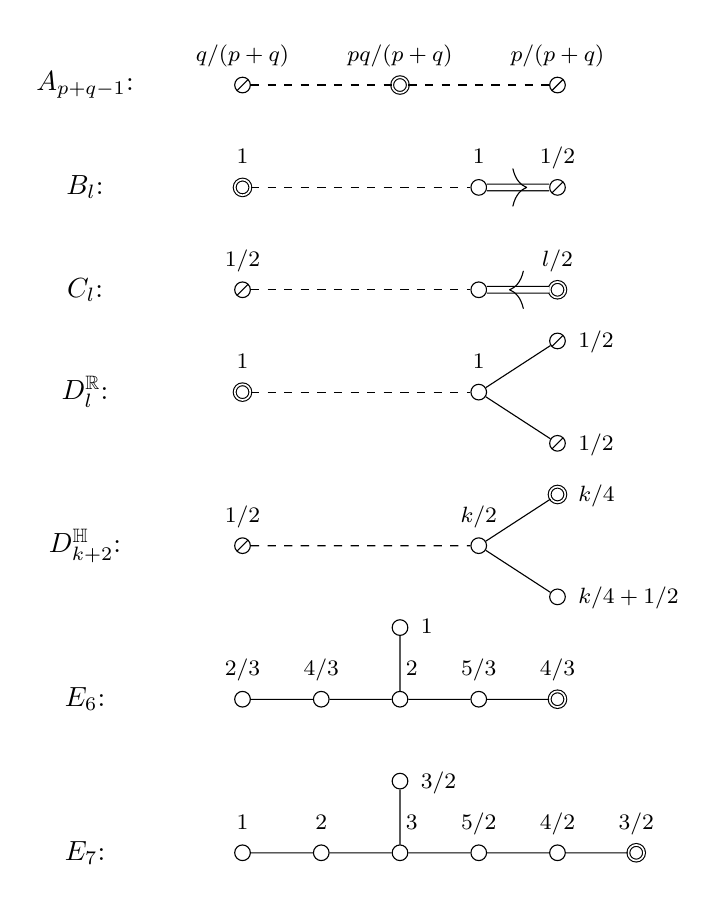
\begin{tikzpicture}[
  yscale=-1.3,
  every node/.style={draw,circle,inner sep=2pt},
  special/.style={double},
  symplectic/.style={forbidden sign},
  every label/.append style={rectangle,font=\footnotesize,
   inner sep=1ex,text depth=1pt},
  decoration={markings,mark=at position 0.7 with {\arrow{>}}},
  doubledynkin/.style={double distance=2pt,postaction=decorate}
  ]
  \node[draw=none] (Atext) at (-1,0) {$A_{p+q-1}$:};
  \node[symplectic] (A1) [label={$q/(p+q)$}] at (1,0) {};
  \node[special] (Ap) [label={$pq/(p+q)$}] at (3,0) {};
  \node[symplectic] (Ak) [label={$p/(p+q)$}] at (5,0) {};
  \draw[dashed] (A1) -- (Ap);
  \draw[dashed] (Ap) -- (Ak);

  \node[draw=none] (Btext) at (-1,1) {$B_{l}$:};
  \node[special] (B1) [label={$1$}] at (1,1) {};
  \node (Blm1) [label={$1$}] at (4,1) {};
  \node[symplectic] (Bl) [label={$1/2$}] at (5,1) {};
  \draw[dashed] (B1) -- (Blm1);
  \draw[doubledynkin] (Blm1) -- (Bl);

  \node[draw=none] (Ctext) at (-1,2) {$C_{l}$:};
  \node[symplectic] (C1) [label={$1/2$}] at (1,2) {};
  \node (Clm1) at (4,2) {};
  \node[special] (Cl) [label={$l/2$}] at (5,2) {};
  \draw[dashed] (C1) -- (Clm1);
  \draw[doubledynkin] (Cl) -- (Clm1);

  \node[draw=none] (DRtext) at (-1,3) {$D_{l}^{\RR}$:};
  \node[special] (DR1) [label={$1$}] at (1,3) {};
  \node (DRlm2) [label={$1$}] at (4,3) {};
  \node[symplectic] (DRlm1) [label=right:{$1/2$}] at (5,2.5) {};
  \node[symplectic] (DRl) [label=right:{$1/2$}] at (5,3.5) {};
  \draw[dashed] (DR1) -- (DRlm2);
  \draw (DRlm1) -- (DRlm2) -- (DRl);

  \begin{scope}[yshift=0.5cm]
   \node[draw=none] (DRtext) at (-1,4) {$D_{k+2}^{\HQ}$:};
   \node[symplectic] (DR1) [label={$1/2$}] at (1,4) {};
   \node (DRlm2) [label={$k/2$}] at (4,4) {};
   \node[special] (DRlm1) [label=right:{$k/4$}] at (5,3.5) {};
   \node (DRl) [label=right:{$k/4+1/2$}] at (5,4.5) {};
   \draw[dashed] (DR1) -- (DRlm2);
   \draw (DRlm1) -- (DRlm2) -- (DRl);
  \end{scope}

  \node[draw=none] (DRtext) at (-1,6) {$E_6$:};
  \node (E61) [label={$2/3$}] at (1,6) {};
  \node (E62) [label={$4/3$}] at (2,6) {};
  \node (E63) [label={\hbox{\hss\quad$2$}}] at (3,6) {};
  \node (E64) [label=right:{$1$}] at (3,5.3) {};
  \node (E65) [label={$5/3$}] at (4,6) {};
  \node[special] (E66) [label={$4/3$}] at (5,6) {};
  \draw (E61) -- (E62) -- (E63) -- (E64);
  \draw (E63) -- (E65) -- (E66);

  \begin{scope}[yshift=0.5cm]
   \node[draw=none] (DRtext) at (-1,7) {$E_7$:};
   \node (E71) [label={$1$}] at (1,7) {};
   \node (E72) [label={$2$}] at (2,7) {};
   \node (E73) [label={\hbox{\hss\quad$3$}}] at (3,7) {};
   \node (E74) [label=right:{$3/2$}] at (3,6.3) {};
   \node (E75) [label={$5/2$}] at (4,7) {};
   \node (E76) [label={$4/2$}] at (5,7) {};
   \node[special] (E77) [label={$3/2$}] at (6,7) {};
   \draw (E71) -- (E72) -- (E73) -- (E74);
   \draw (E73) -- (E75) -- (E76) -- (E77);
  \end{scope}
 \end{tikzpicture}
\]
Legend (and comparison with \cite{Del_ShimVar}):
\begin{itemize}
 \item nodes are represented by circles
  \tikz \node[draw,circle,inner sep=2pt] {};
  (bars in \cite{Del_ShimVar});
 \item special nodes are represented by double circles
  \tikz \node[draw,circle,inner sep=2pt,double] {};
  (circled nodes in \cite{Del_ShimVar});
 \item symplectic nodes are represented by slashed circles
  % TODO define symplectic
  \tikz \node[draw,circle,inner sep=2pt,forbidden sign] {};
  (underlined nodes in \cite{Del_ShimVar}).
\end{itemize}
The rational number above a node $\omega$ is $\langle \mu,\omega \rangle$,
where $\mu$ is the cocharacter corresponding to the special node,
and $\omega$ is identified with
the fundamental representation that it corresponds with.

In diagram~$A_{p+q-1}$ it is the $p$-th node that is special.
The diagram~$D_{k+2}^{\HQ}$ is required to satisfy $k + 2 \ge 5$.
Observe that diagrams of type~$E_8$, $F_4$, and~$G_2$ do not occur:
they do not have special nodes.
The diagrams of type~$E_6$ and~$E_7$ do not have symplectic nodes.

\begin{definition} % {{{-2
 \label{deligne-dynkin-diagram}
 A \emph{Deligne--Dynkin diagram} is a pair $(\Delta, \mu)$, where
 \begin{itemize}
  \item $\Delta$ is a Dynkin diagram
   equipped with an action of~$\Gal(\QQbar/\QQ)$;
  \item $\mu$ is a non-empty subset of~$\Delta$
   (that is not required to be $\Gal(\QQbar/\QQ)$-stable)
   consisting of at most~$1$ node per connected component of~$\Delta$
   that must be a special node
   (see \cref{table-deligne-dynkin-diagrams}).
 \end{itemize}
 The Deligne--Dynkin diagram $(\Delta, \mu)$ is called \emph{irreducible}
 if $\pi_0(\Delta)$ is irreducible as $\Gal(\QQbar/\QQ)$-set.
\end{definition}

\begin{definition} % {{{-2
 \label{symplectic-nodes-deligne-dynkin-diagram}
 Let $(\Delta, \mu)$ be an irreducible Deligne--Dynkin diagram.
 The \emph{subset of symplectic nodes} attached to $(\Delta, \mu)$
 is the maximal subset $S \subset \Delta$ defined by the following conditions:
 \begin{enumerate}
  \item For every special node $\alpha \in \mu \subset \Delta$,
   let $\Delta_\alpha$ denote the connected component of~$\Delta$
   that contains~$\alpha$.
   Then $S \cap \Delta_\alpha$ consists only of
   symplectic nodes of~$\Delta_\alpha$ with respect to~$\alpha$.
   (See also \cref{table-deligne-dynkin-diagrams}.)
  \item The set $S$ is stable under the action of $\Gal(\QQbar/\QQ)$.
 \end{enumerate}
\end{definition}

\begin{definition} % {{{-2
 An irreducible Deligne--Dynkin diagram is \emph{symplectic}
 if its subset of symplectic nodes is non-empty.
\end{definition}

\paragraph{The type of $\Delta,\mu)$} % {{{-2
Let $(\Delta, \mu)$ be an irreducible Deligne--Dynkin diagram.
The \emph{type} of $(\Delta, \mu)$ is
the type of a connected component of~$\Delta$.
If $(\Delta, \mu)$ is symplectic, then its type is classical:
$A_n$,~$B_n$, $C_n$, or~$D_n$.
Conversely, if the type of $(\Delta, \mu)$ is $A_n$,~$B_n$, or~$C_n$,
then $(\Delta, \mu)$ is symplectic.
The case where the type of $(\Delta, \mu)$ is $D_n$ requires more attention.

Assume the type of $(\Delta, \mu)$ is $D_n$, with $n \ge 5$.
For every special node $\alpha \in \mu \subset \Delta$,
let $\Delta_\alpha$ be the connected component of~$\Delta$
that contains~$\alpha$.
The pair $(\Delta, \alpha)$ is of type~$D_n^\RR$ or~$D_n^\HQ$
according to the diagrams listed in \cref{table-deligne-dynkin-diagrams}.
One readily verifies that $(\Delta, \mu)$ is symplectic if and only if
one of the following conditions holds:
\begin{itemize}
 \item for every special node~$\alpha$, the pair $(\Delta, \alpha)$
  is of type $D_n^\RR$; or
 \item for every special node~$\alpha$, the pair $(\Delta, \alpha)$
  is of type $D_n^\HQ$.
\end{itemize}
We say that it is of type~$D_n^\RR$ (resp.~$D_n^\HQ$)
if the former (resp.~the latter) condition holds.

Now assume that $(\Delta, \mu)$ is of type $D_4$.
Let $V$ be the subset of extremal nodes of~$\Delta$,
let $\bar\mu$ be the $\Gal(\QQbar/\QQ)$-closure of~$\mu$,
and let $S$ be the subset of symplectic nodes attached to $(\Delta,\mu)$.
Observe that $S \subset V$,
and $S$ meets every compontent of~$\Delta$ in $0$,~$1$, or~$2$ nodes.
(In other words, the degree of~$S$ over $\pi_0(\Delta)$ at most~$2$.)
In the former case, $S$ is empty, and $(\Delta, \mu)$ is not symplectic.
In the latter two cases $V = \bar\mu \sqcup S$, by the maximality of~$S$.
We say that $(\Delta, \mu)$ has type $D_4^\RR$
if $\deg(\bar\mu) = 1$ and $\deg(S) = 2$,
while $(\Delta, \mu)$ has type $D_4^\HQ$
if $\deg(\bar\mu) = 2$ and $\deg(S) = 1$.


\begin{proposition} % {{{-2
 Let $(\Delta_1, \mu_1)$ and $(\Delta_2, \mu_2)$ be
 two symplectic Deligne--Dynkin diagrams
 and suppose that there is an isomorphism
 $\phi_0 \colon \pi_0(\Delta_1) \to \pi_0(\Delta_2)$
 and for each prime number~$\ell$
 a $\Gal(\QQlbar/\QQl)$-equivariant bijection
 $\phi_\ell \colon \Delta_1 \to \Delta_2$ identifying $\mu_1$ with~$\mu_2$
 such that $\pi_0(\phi_\ell) = \phi_0$.
 Then $(\Delta_1, \mu_1) \cong (\Delta_2, \mu_2)$.
\end{proposition}

% {{{-1 Footer
\printbibliography

\end{document}
